The $Z+$jets background has a very different $E_{\text{T}}^{\text{miss}}$ signature than VBF Higgs events. This is because while both processes contain neutrinos, the $Z+$jets neutrinos have a lower average transverse energy. The BDT trained to discriminate between VBF signal events and the $Z+$jets background uses a range of $E_{\text{T}}^{\text{miss}}$ variables and cutting on this trained discriminant rather directly on $E_{\text{T}}^{\text{miss}}$ provides an enhanced purity. The training and results from the BDT are described in the next subsection. Note that the following results from substantial optimization on training inputs and techniques. The final BDT has high discrimination, no under or overtraining, and utilizes variables which are well-modeled and not highly correlated to one another.  
The BDT is trained using $e\mu+\mu e$ events after the VBF selection and includes the signal region cuts including that on $n_{jets}$, $b$-veto, OLV, CJV, $m_{jj}$ and $\Delta Y_{jj}$. In this way, the phase space in which we train the BDT is exactly the same as the one where we apply it. The training includes only the $Z\rightarrow\tau\tau$ background and the VBF signal. The training corresponds to $\approx$ 5,000 $Z\tau\tau$ events and $\approx$100,000 VBF events.

The TMVA BDTG interface is used to train and test the BDT. The optimal parameters were found through a scan of reasonable values and the final set is summarized in Table~\ref{tab:ZBDTparameters}.

\begin{table}[htbp!]
\centering
\begin{tabular}{|l|c|c|}
\hline
Parameter                                    & Value    & Range     \\
\hline
Boosting algorithm                           & Gradient & --        \\
Maximum tree depth                           &  22      & [3,10,22,30]    \\
Number of trees                              &  1000    & [200,1000,10000] \\
Minimum number of events requires per mode   &  5\%     & [5\%]\\
Number of cuts                               &  7       & [3,5,7,9]  \\
\hline
\end{tabular}
\caption{BDT parameters used for the $Z\rightarrow\tau\tau$ training.} 
\label{tab:ZBDTparameters}
\end{table}

For this BDT, we aim to take advantage of the different $E_{\text{T}}^{\text{miss}}$ distributions in $Z\rightarrow\tau\tau$ and VBF MC events. We train the BDT using multiple different $E_{\text{T}}^{\text{miss}}$ variables to maximize discrimination and then cut on the BDT output variable. The optimal analysis uses $\ensuremath{E_{\text{T}}^{\text{miss, significance}}}$, $\ensuremath{E_{\text{T}}^{\text{miss, track}}}$, $\ensuremath{E_{\text{T,rel}}^{\text{miss}}}$, $\ensuremath{E_{\text{T,rel}}^{\text{miss, track}}}$, $\ensuremath{\Delta\phi_{\ell\ell,E_{\text{T}}^{\text{miss, track}}}}$, and $\ensuremath{\Delta\phi_{\ell\ell,E_{\text{T}}^{\text{miss}}}}$. Relative $E_{\text{T}}^{\text{miss}}$ is defined as $E_{\text{T}}^{\text{miss}} * \sin(|\Phi_{E_{\text{T}}^{\text{miss}}}\Phi_{jet}|)$, $\ensuremath{E_{\text{T}}^{\text{miss, track}}}$ is calculated from tracking detectors while $E_{\text{T}}^{\text{miss}}$ is calculated from calorimeter deposits. The $\ensuremath{E_{\text{T}}^{\text{miss, significance}}}$ variable differentiates between $E_{\text{T}}^{\text{miss}}$ from electroweak and strong interactions \cite{JETEtmiss}. Figure~\ref{fig:ZjetsBDTinput} and~\ref{fig:ZjetscorrSB} demonstrate the input distributions used to train the BDT and their correlations.

\begin{figure}[!htbp]
    \centering
    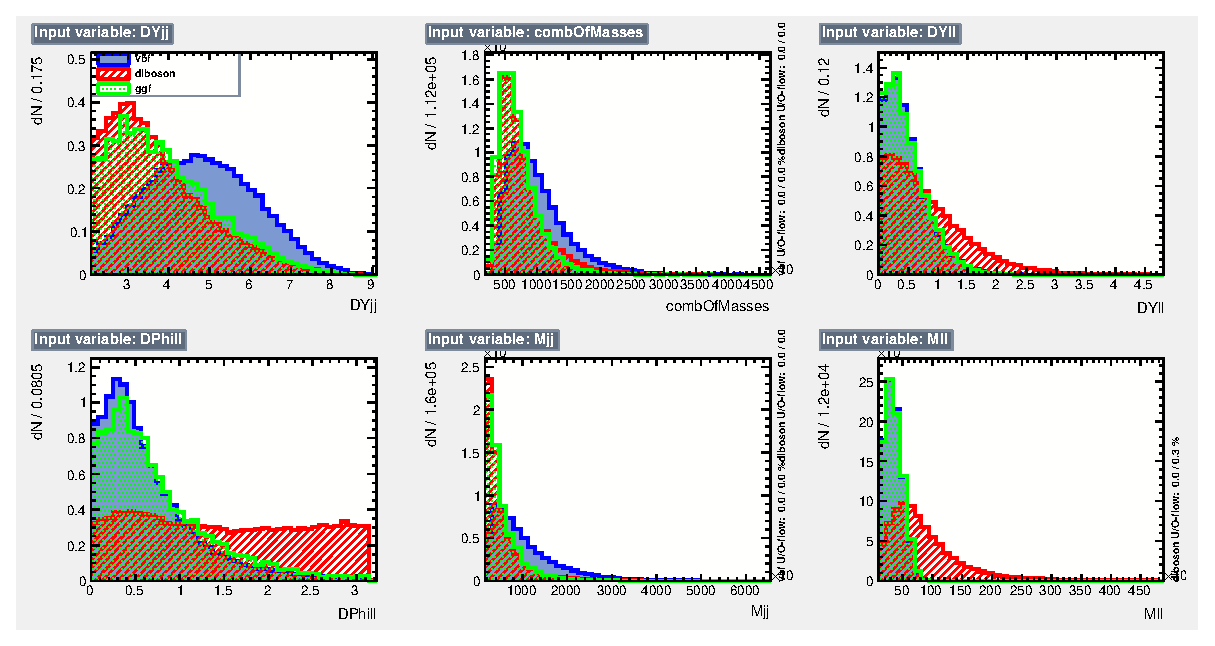
\includegraphics[width=0.85\linewidth]{Pictures/variables_id_c1.eps}
    \caption{Distributions of input variables to $Z\rightarrow\tau\tau$ BDT. Samples are normalized to even numbers of background and signal events. Signal represents $Z\rightarrow\tau\tau$ and background VBF Higgs.}.
    \label{fig:ZjetsBDTinput}
\end{figure}
\begin{figure}[!htbp]
\centering
  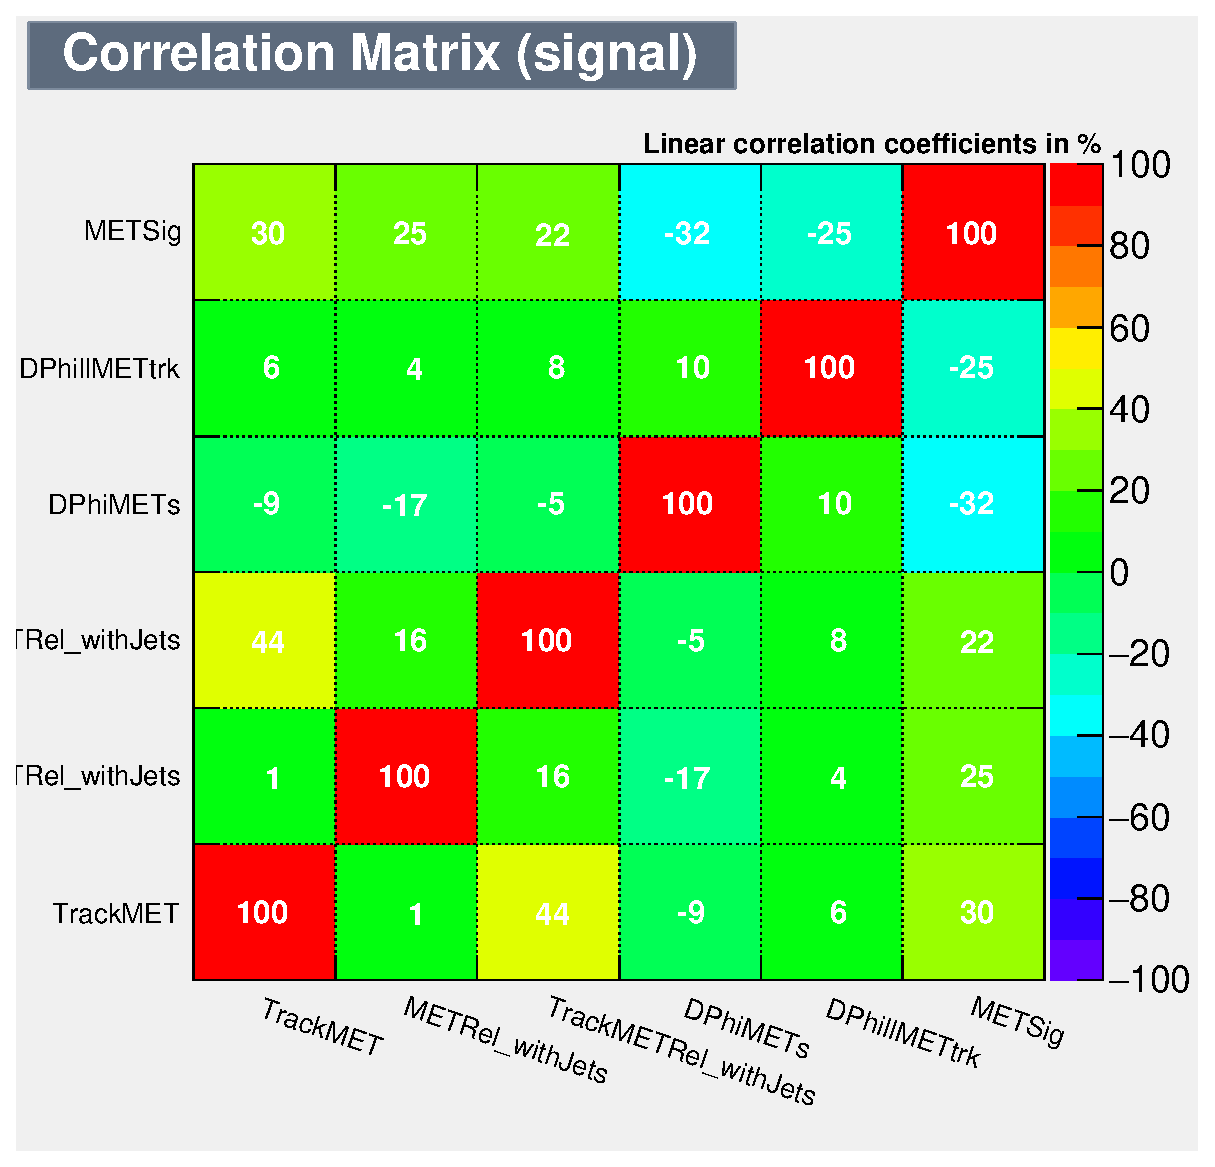
\includegraphics[width=.4\linewidth]{Pictures/CorrelationMatrixS.eps}
  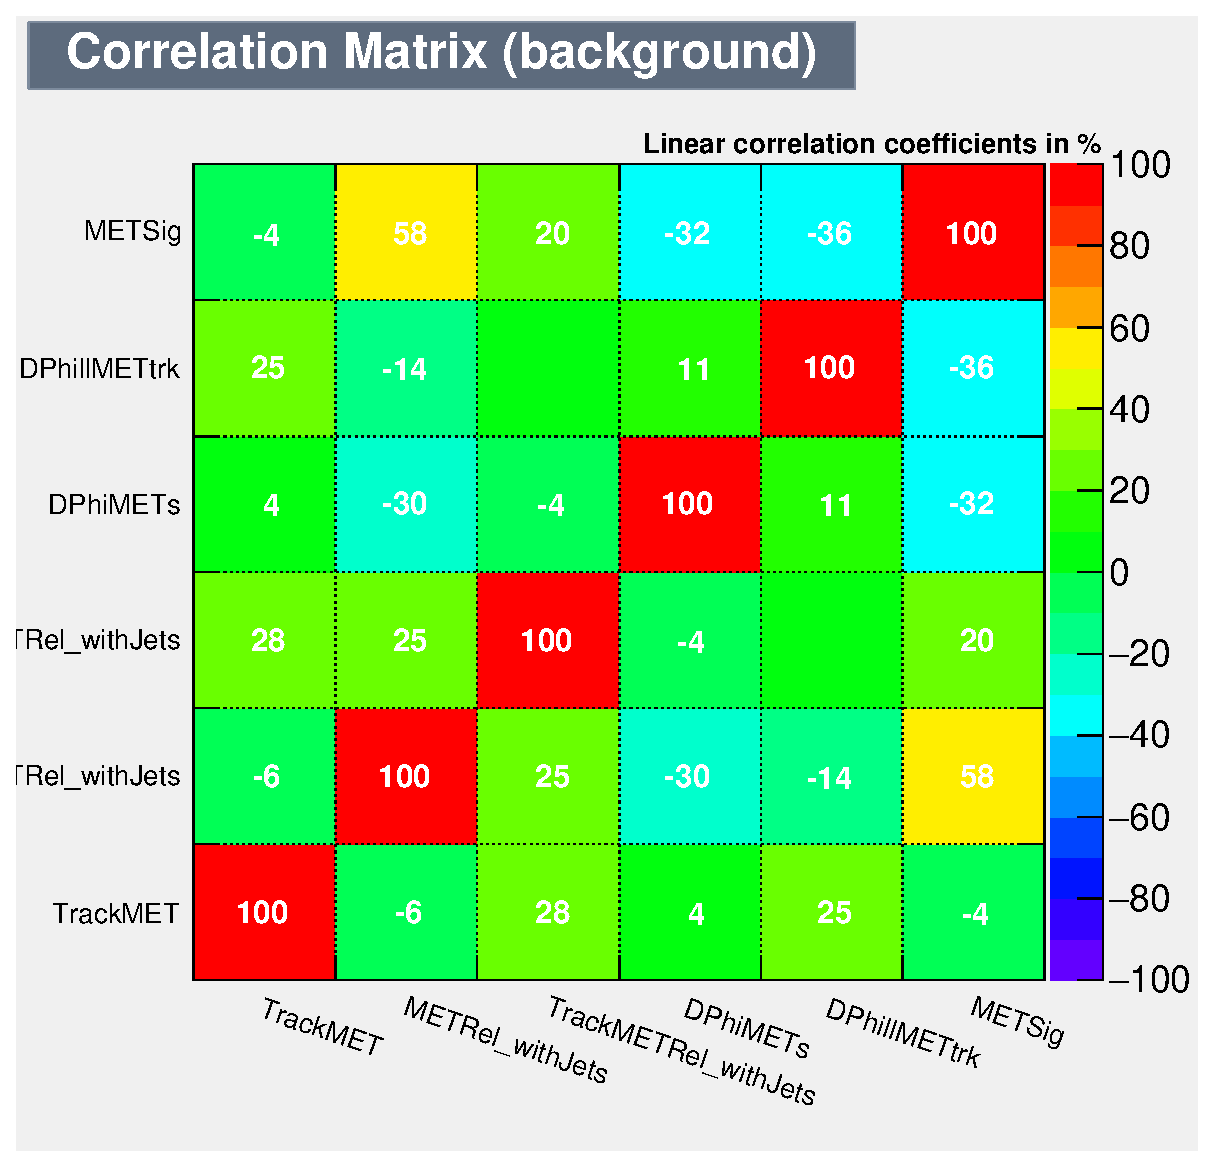
\includegraphics[width=.4\linewidth]{Pictures/CorrelationMatrixB.eps}
\caption{Correlations of input variables to $Z\rightarrow\tau\tau$ BDT. Signal represents $Z\rightarrow\tau\tau$ and background VBF Higgs.}
\label{fig:ZjetscorrSB}
\end{figure}
The BDT training successfully separates $Z\rightarrow\tau\tau$ and VBF signal. In order to quantify the discrimination we use the integrated-ROC calculated through TMVA and find an optimal value of 0.897. For signal and background, we find KS-test values of 0.062 and 0.286, and so no evidence of over-training. Figures~\ref{fig:ZjetsBDTresult} and \ref{fig:ZjetsBDTresult2} show BDT results applied to normalized samples of $Z\rightarrow\tau\tau$ and VBF signal and to all weighted background and signal events. 

\begin{figure}[!htbp]
 \centering
  \includegraphics[width=.45\linewidth]{Pictures/ZttBDT/overtrain_BDTG.eps}
\caption{Normalized samples of $\Ztt$ (signal) and VBF (background) plotted over BDT output distribution, overlaid testing and training samples shown.}
\label{fig:ZjetsBDTresult}
\end{figure}
\begin{figure}
\centering
  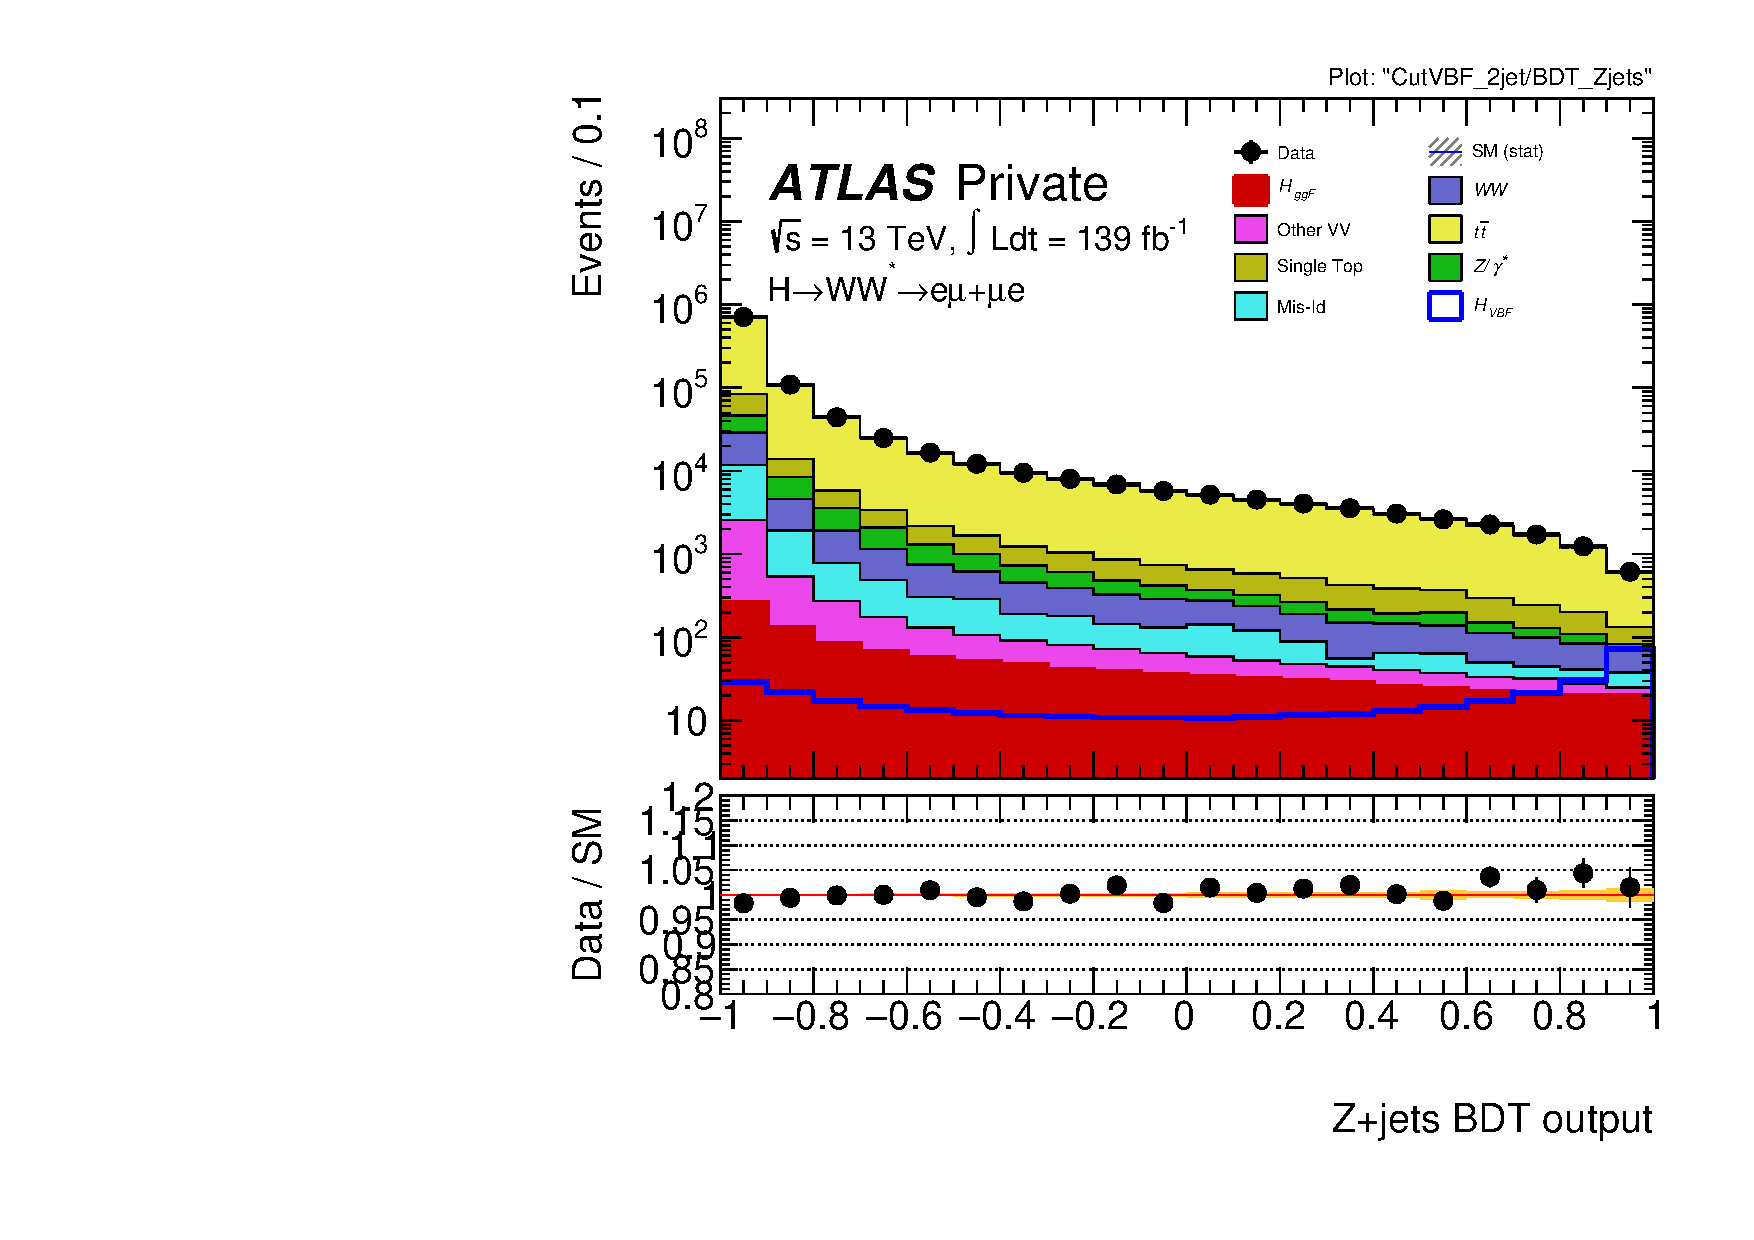
\includegraphics[width=.6\linewidth]{Pictures/run2-emme-CutVBF_2jet-BDT_Zjets-log.pdf}
\caption{Weighted samples of VBF signal, $\Ztt$, and all other backgrounds plotted over BDT$_{\Ztt}$ after pre-selection cuts}
\label{fig:ZjetsBDTresult2}
\end{figure}

Figure~\ref{fig:ZjetsBDTinterpret} shows distributions of all samples against $\Ztt$ BDT output in the signal region after the cut on BDT$_{\Ztt}$ is applied. Cuts on the BDT output variable are chosen to increase significance while also maintaining high signal statistics. Cutting on a BDT output value of 0.5 eliminates $60\%$ of $\Ztt$ background, or $\approx 450$ events, and only $6\%$ of signal events. This cut is also tested on truth samples to validate that applying it does not affect the fiducial phase space. 

\begin{figure}[!htbp]
\centering
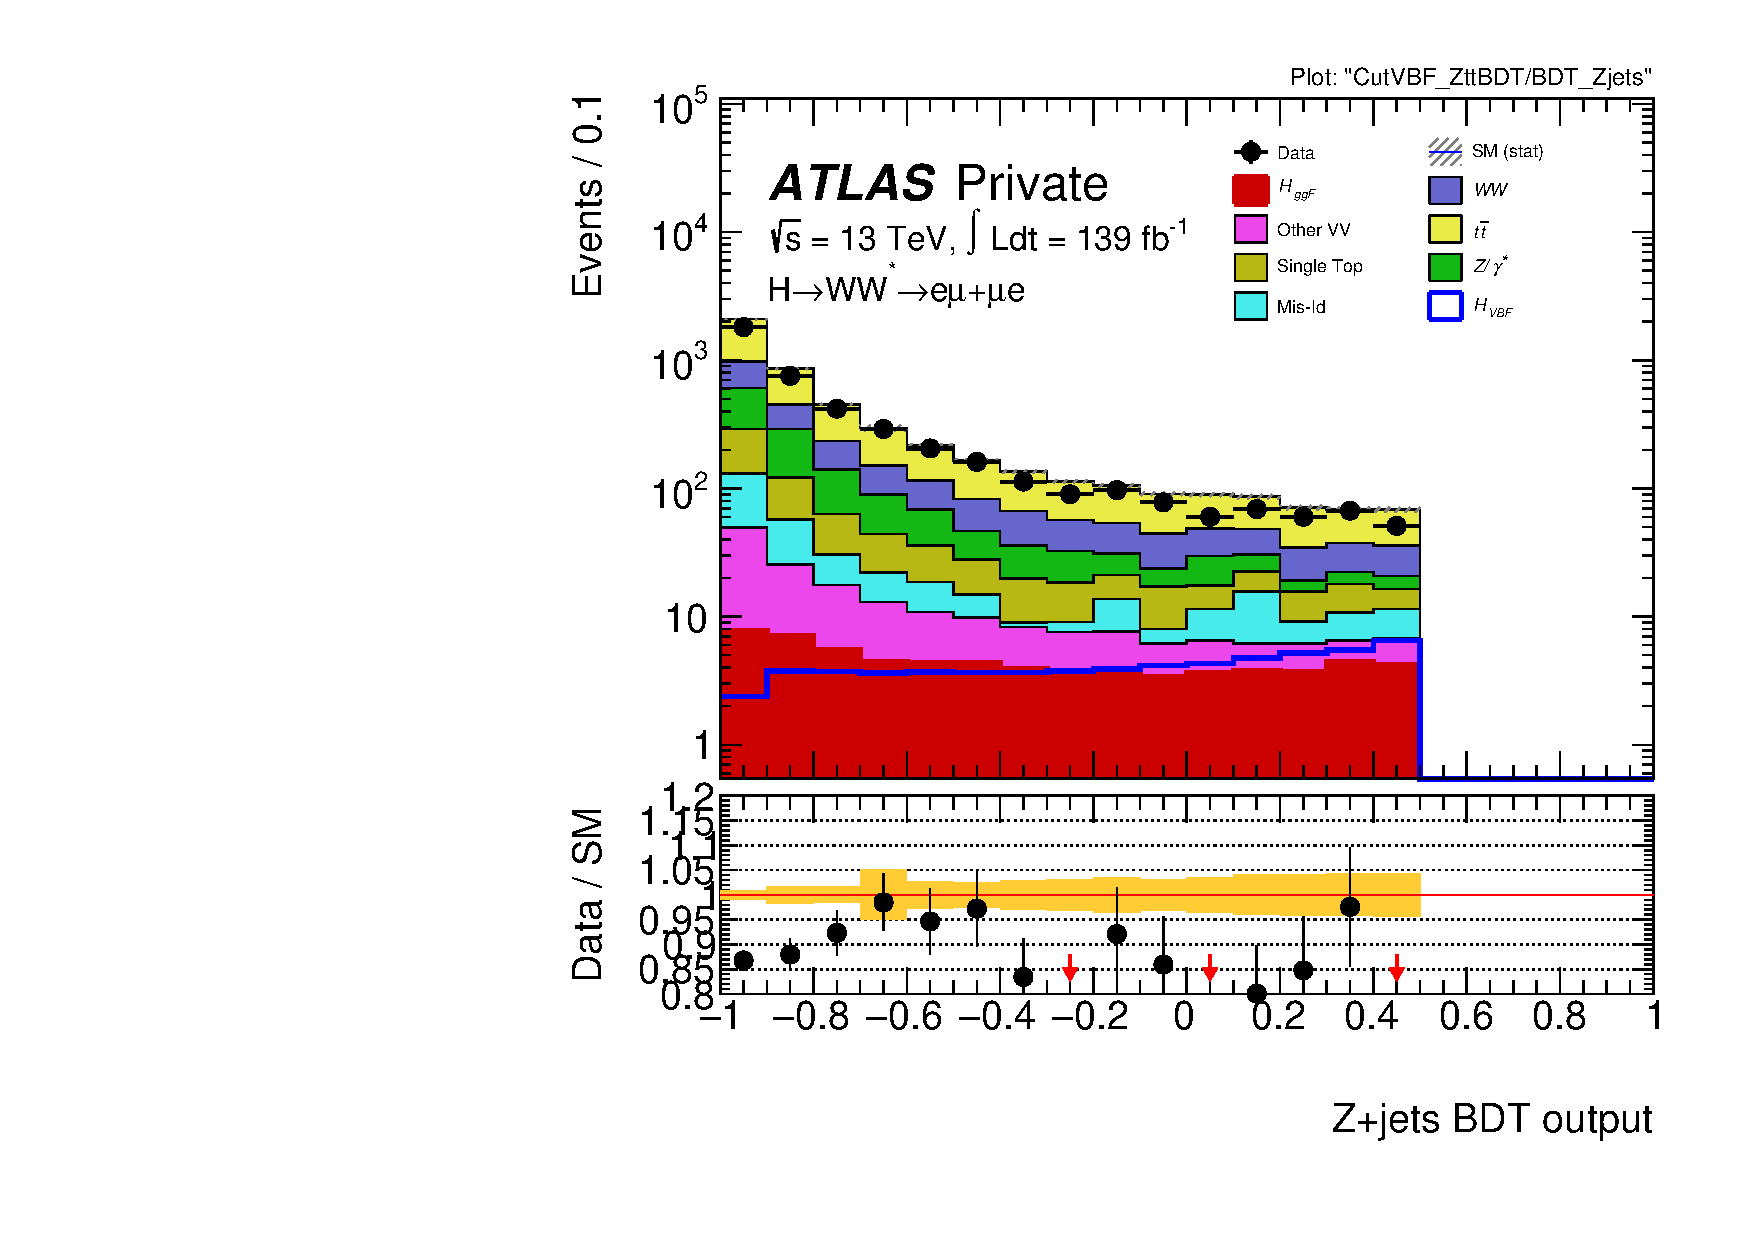
\includegraphics[width=.6\linewidth]{Pictures/ZttBDT/run2-emme-CutVBF_ZttBDT-BDT_Zjets-log.pdf}
\caption{Full weighted samples plotted over the $\Ztt$ BDT output in the signal region after cutting on BDT$_\Ztt$}
\label{fig:ZjetsBDTinterpret}
\end{figure}

Four different iterations of signal and $\Ztt$ control region definitions are used in the simultaneous fit with Asimov data, and results are examined with and without systematic uncertainties. The signal region is defined as described in the main text with at least 2 jets ($n_{jets}>=2$), a $b$-veto, $\Ztt$ veto, central-jet-veto (CJV), outside-lepton-veto (OLV), and cuts on $m_{jj}>200$ GeV and on the rapidity difference between the two jets ($\Delta Y_{jj}>2.1$). The $\Ztt$ control region is defined in two different ways--first, as in the text with signal region cuts requiring 2 jets, a b-veto, OLV and CJV as well as additional cuts reversing the $\Ztt$ veto with $66.2$~GeV $< m_{\tau\tau}< 116.2 $~GeV. An alternative definition of the $\Ztt$ control region is within the signal region with orthogonality defined with a cut on the $\Ztt$ BDT output. The four tested configurations are described in Table~\ref{tab:ZBDTfitconditions}. 

\begin{table}[h!]
\centering
\resizebox{\textwidth}{!}{
\begin{tabular}{|c|c|c|c|}
\hline
Configuration name      & Signal region   & $\Ztt$ control region & $\Ztt$ control region axis     \\
\hline
\textbf{A}                           & default & $\Ztt$ CR & $m_T$  \\
\textbf{B}                           & default + BDT$_{\Ztt}>0.5$ & $\Ztt$ CR & $m_T$    \\
\textbf{C}                           & Signal region + BDT$_{\Ztt}>0.5$ & Signal region + BDT$_{\Ztt}<0.5$ & BDT$_{\Ztt}$ \\
\textbf{D}			    & Signal region + BDT$_{\Ztt}>0.0$ & Signal region + BDT$_{\Ztt}<0.0$     & BDT$_{\Ztt}$\\
\hline
\end{tabular}}
\caption{Four testing conditions for signal and $\Ztt$ control region definitions.}
\label{tab:ZBDTfitconditions}
\end{table}

The four testing conditions were included in a simultaneous fit with other regions defined as detailed in the main text. These studies are conducted with $V20$ pxAODS and associated $V20$ trained BDTs. We also perform the fit with Asimov data only. First, the fit was performed without any experimental or theoretical uncertainties, then experimental uncertainties were added and each parameter was tested again. Table~\ref{tab:ZBDTstatonly} summarizes the uncertainty determined on each fit parameter when only statistical uncertainties are considered, using the testing conditions defined in Table~\ref{tab:ZBDTfitconditions}. 

\begin{table}[h!]
\centering
\begin{tabular}{|l|c|c|c|c|}
\hline
     & \textbf{A}   & \textbf{B} & \textbf{C} & \textbf{D}     \\
\hline
$\mu_{VBF}$ & $ 0.171$ &  $0.165$ & $0.143$ & $0.169$\\
$\mu_{\Ztt}$ & $ 0.005$ & $0.038$ & $0.020$ & $0.052$\\
$\mu_{ggF}$ & $0.485$ & $0.451$ & $ 0.294$ & $0.469$\\
$\mu_{ggF1}$ & $0.449$ & $0.430$ & $0.269$ & $ 0.439$\\
$\mu_{ggF2}$ & $0.151$ & $0.172$ & $0.129$ & $0.172$\\
$\mu_{TopWW}$ & $0.013$ & $0.014$ & $0.003$ & $0.010$ \\
\hline
\end{tabular}
\caption{Signal strength uncertainty for each fit parameter in a stat-only fit using four $\Ztt$ control region conditions.}
\label{tab:ZBDTstatonly}
\end{table}
 
These studies show no large gains from using conditions \textbf{B} or \textbf{D} instead of the default of \textbf{A} in which no BDT is used at all. Using condition \textbf{C} may have some positive effect from use of the BDT as both a binning cut to determine the $\Ztt$ background region within the signal region and VBF signal region itself and an axis used in the total fit. However, adding systematics to this affects the overall results differently.  

\begin{table}[h!]
\centering
\begin{tabular}{|l|c|c|c|c|}
\hline
     & \textbf{A}   & \textbf{B} & \textbf{C} & \textbf{D}     \\
\hline
$\mu_{VBF}$ & $0.202$ &  $0.196$ & $0.196$ & $0.195$\\
$\mu_{\Ztt}$ & $0.019$ & $0.056$ & $0.054$ & $0.076$\\
$\mu_{ggF}$ & $0.645$ & $0.646$ & $0.648$ & $0.670$\\
$\mu_{ggF1}$ & $0.565$ & $0.566$ & $0.574$ & $0.587$\\
$\mu_{ggF2}$ & $0.407$ & $0.323$ & $0.323$ & $0.272$\\
$\mu_{TopWW}$ & $0.018$ & $0.017$ & $0.018$ & $0.015$ \\
\hline
\end{tabular}
\caption{Signal strength uncertainty for each fit parameter in a stat-only fit using four $\Ztt$ control region conditions.}
\label{tab:ZBDTstatsys}
\end{table}

Overall results are not changed significantly by the addition of the $BDT_{\Ztt}$ parameter in the overall fit when systematic uncertainties are taken into account. The low statistics of $\Ztt$ events in its designated control region (within or outside the signal region) likely cause the higher uncertainties when this cut is used. After the conclusion of these studies configuration \textbf{A} was chosen for the analysis. 

%The plots following show results from the each iteration- first correlation plots then plots showing the $\Ztt$, WW and top regions after each type of fit.
%\begin{figure}[!htbp]
%\centering
%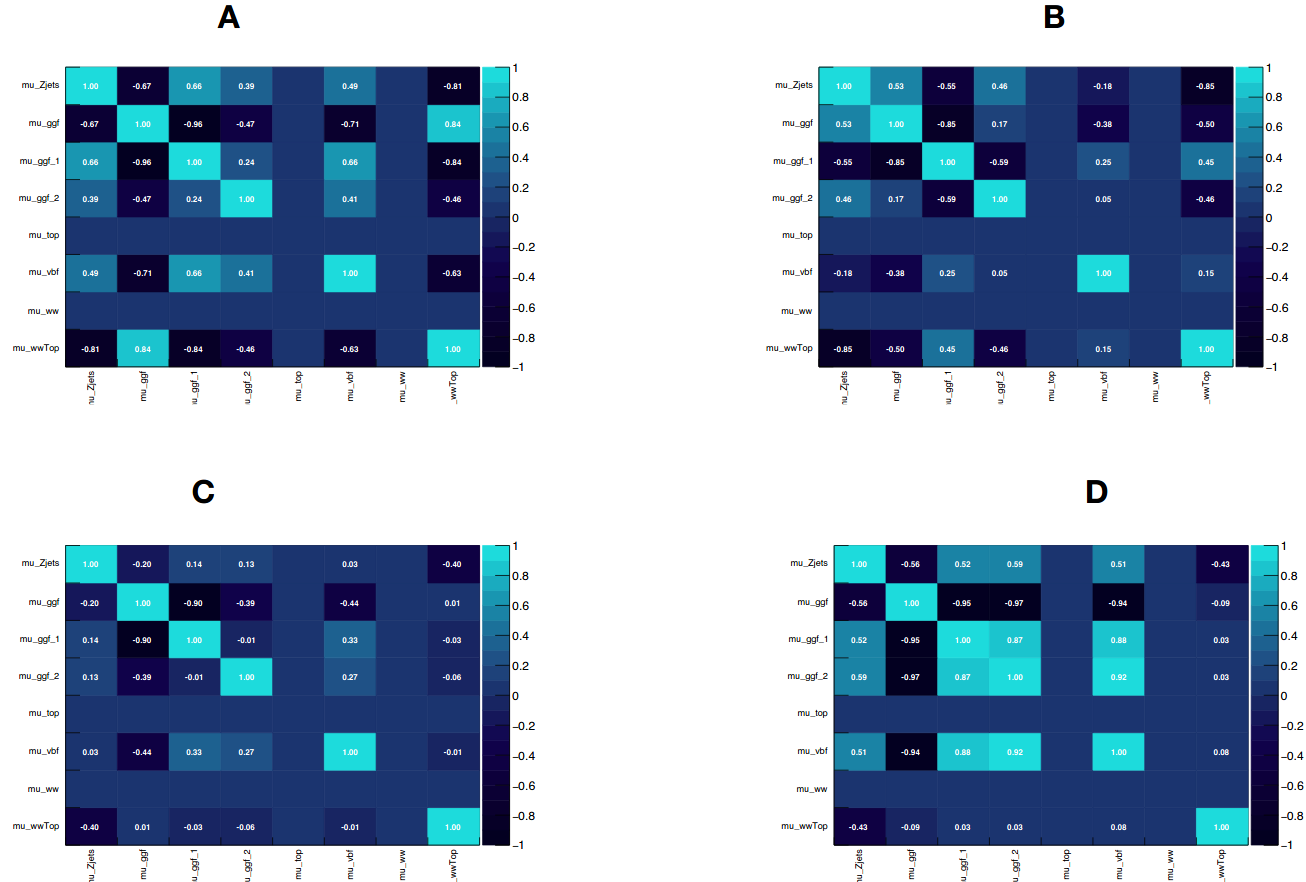
\includegraphics[width=.9\linewidth]{Pictures/ZttBDT/correlations.png}
%\caption{Correlations on fit parameters for each of four region parameters}
%\label{fig:ZjetsBDTcorrelation}
%\end{figure} 
%%
%\begin{figure}[!htbp]
%\centering
%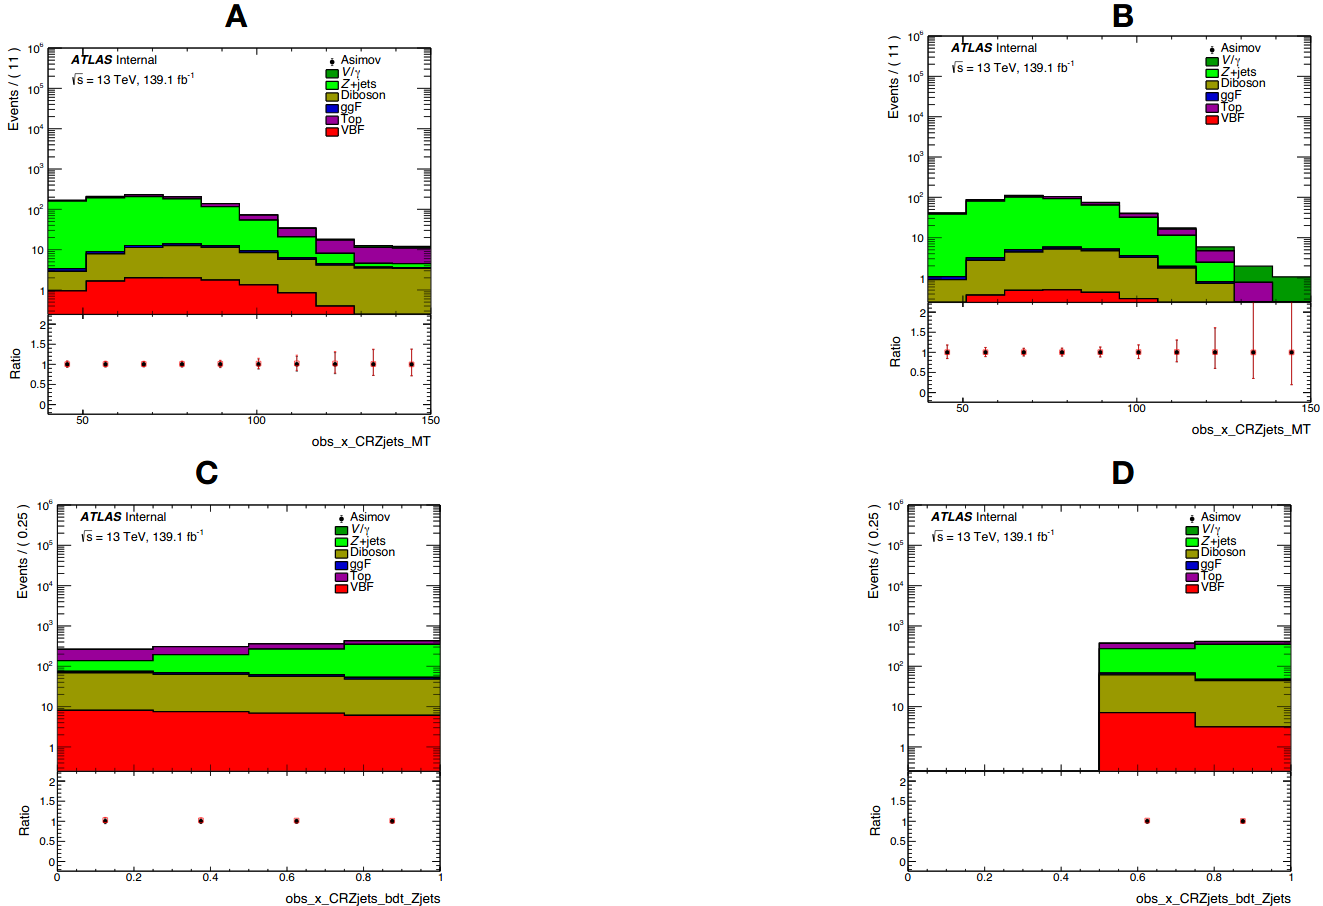
\includegraphics[width=.9\linewidth]{Pictures/ZttBDT/ZttCR.png}
%\caption{$\Ztt$ distributions for each of four region parameters}
%\label{fig:ZjetsBDTZttCR}
%\end{figure} 
%
%\begin{figure}[!htbp]
%\centering
%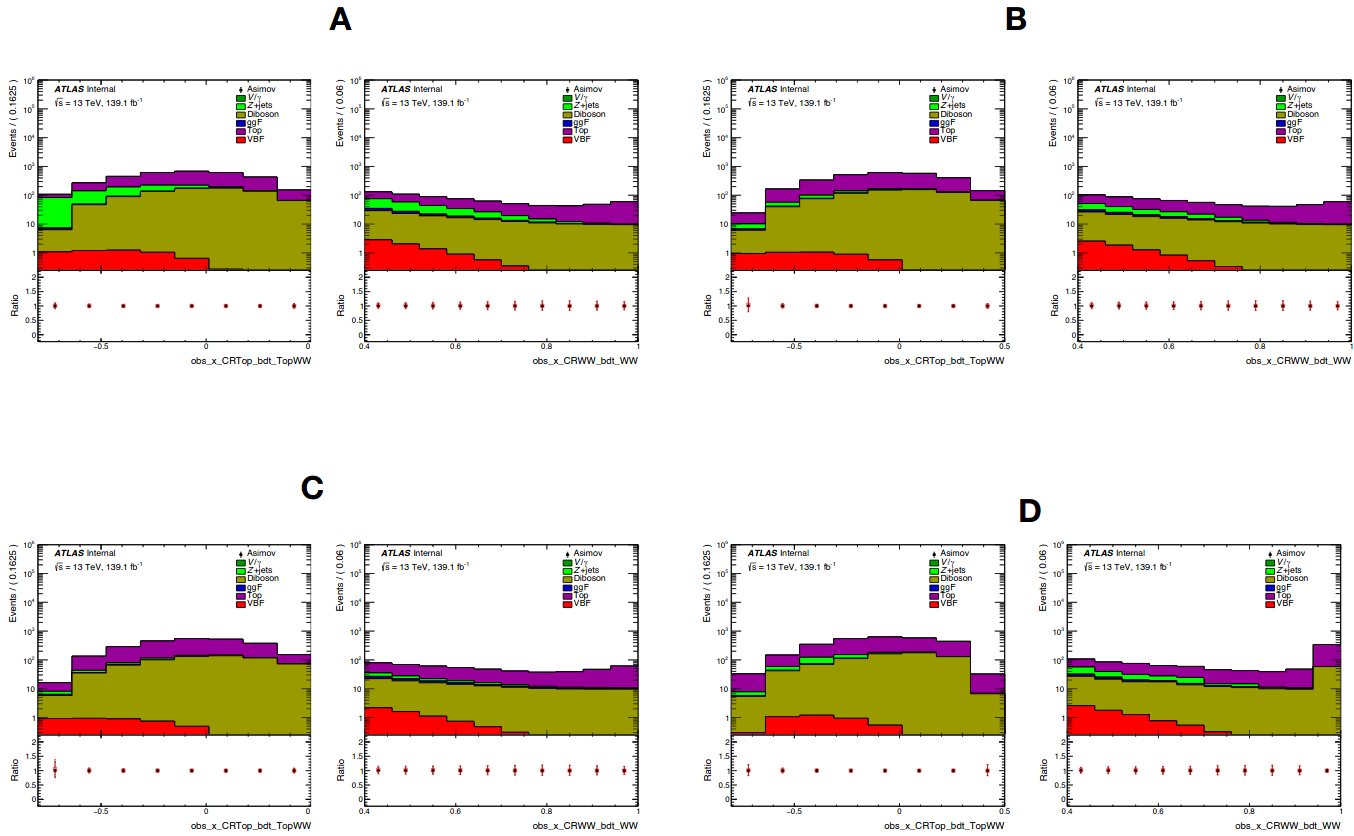
\includegraphics[width=.9\linewidth]{Pictures/ZttBDT/TopWWCR.png}
%\caption{Top and WW distributions for each of four region parameters}
%\label{fig:ZjetsBDTTopWWCR}
%\end{figure} 

%\begin{figure}[!htbp]
%\centering
  %\includegraphics[width=.4\linewidth]{Pictures/overtrain_BDTG.eps}
%  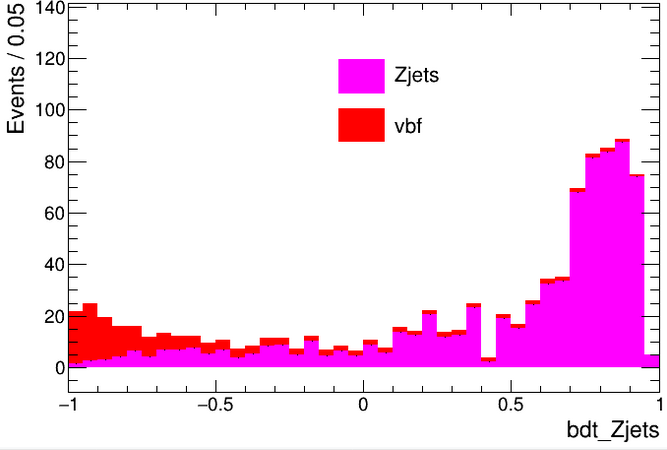
\includegraphics[width=.4\linewidth]{Pictures/weightedZjetsVBF.png}
%\caption{Weighted, normalized samples of $Z\rightarrow\tau\tau$ (signal) and VBF (background) plotted over BDT output distribution on left, overlaid testing and training samples shown. On right, full weighted samples of $Z\rightarrow\tau\tau$ and VBF signal plotted over BDT output distributions.}
%\label{fig:ZjetsBDTresult}
%\end{figure}

%Finally, we can test how other background samples distribute with the $Z\rightarrow\tau\tau$ BDT output variable and optimize results from cutting on this variable. The following plot \ref{fig:ZjetsBDTinterpret} shows distribution of all backgrounds as well as signal with $Z\rightarrow\tau\tau$ BDT output. We aim to increase significance while also keeping as much signal sample as possible for keep high statistics. To accomplish this we cut at a BDT output value of 0.5, in this way we eliminate $60\%$ of $Z\rightarrow\tau\tau$ background, or $\approx 450$events, and only $6\%$ of signal events. We have also tested this cut on truth samples to validate that applying this cut does not affect our fiducial phase space. 
%\begin{figure}[!htbp]
%\centering
%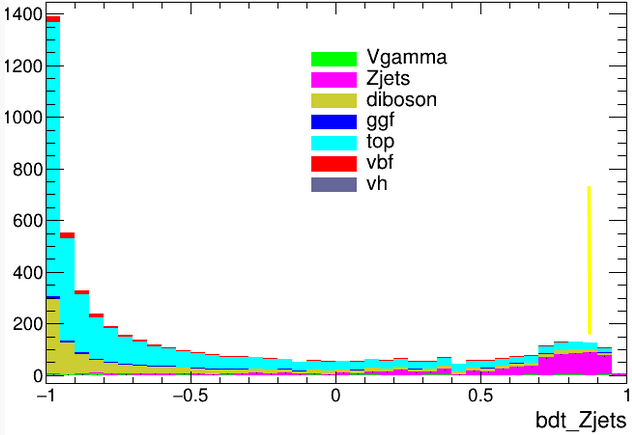
\includegraphics[width=.4\linewidth]{Pictures/weightedZjetsAll.png}
%\caption{Full weighted samples of all signal and background plotted over BDT output distributions}
%\label{fig:ZjetsBDTintepret}
%\end{figure}

%The BDT that discriminates VBF signal and $Z+$jets is applied in the $Z+$jets control region to maintain orthogonality. This further increases purity in the control region. This distribution is shown in the following plot.
%\begin{figure}[!htbp]
%\centering
%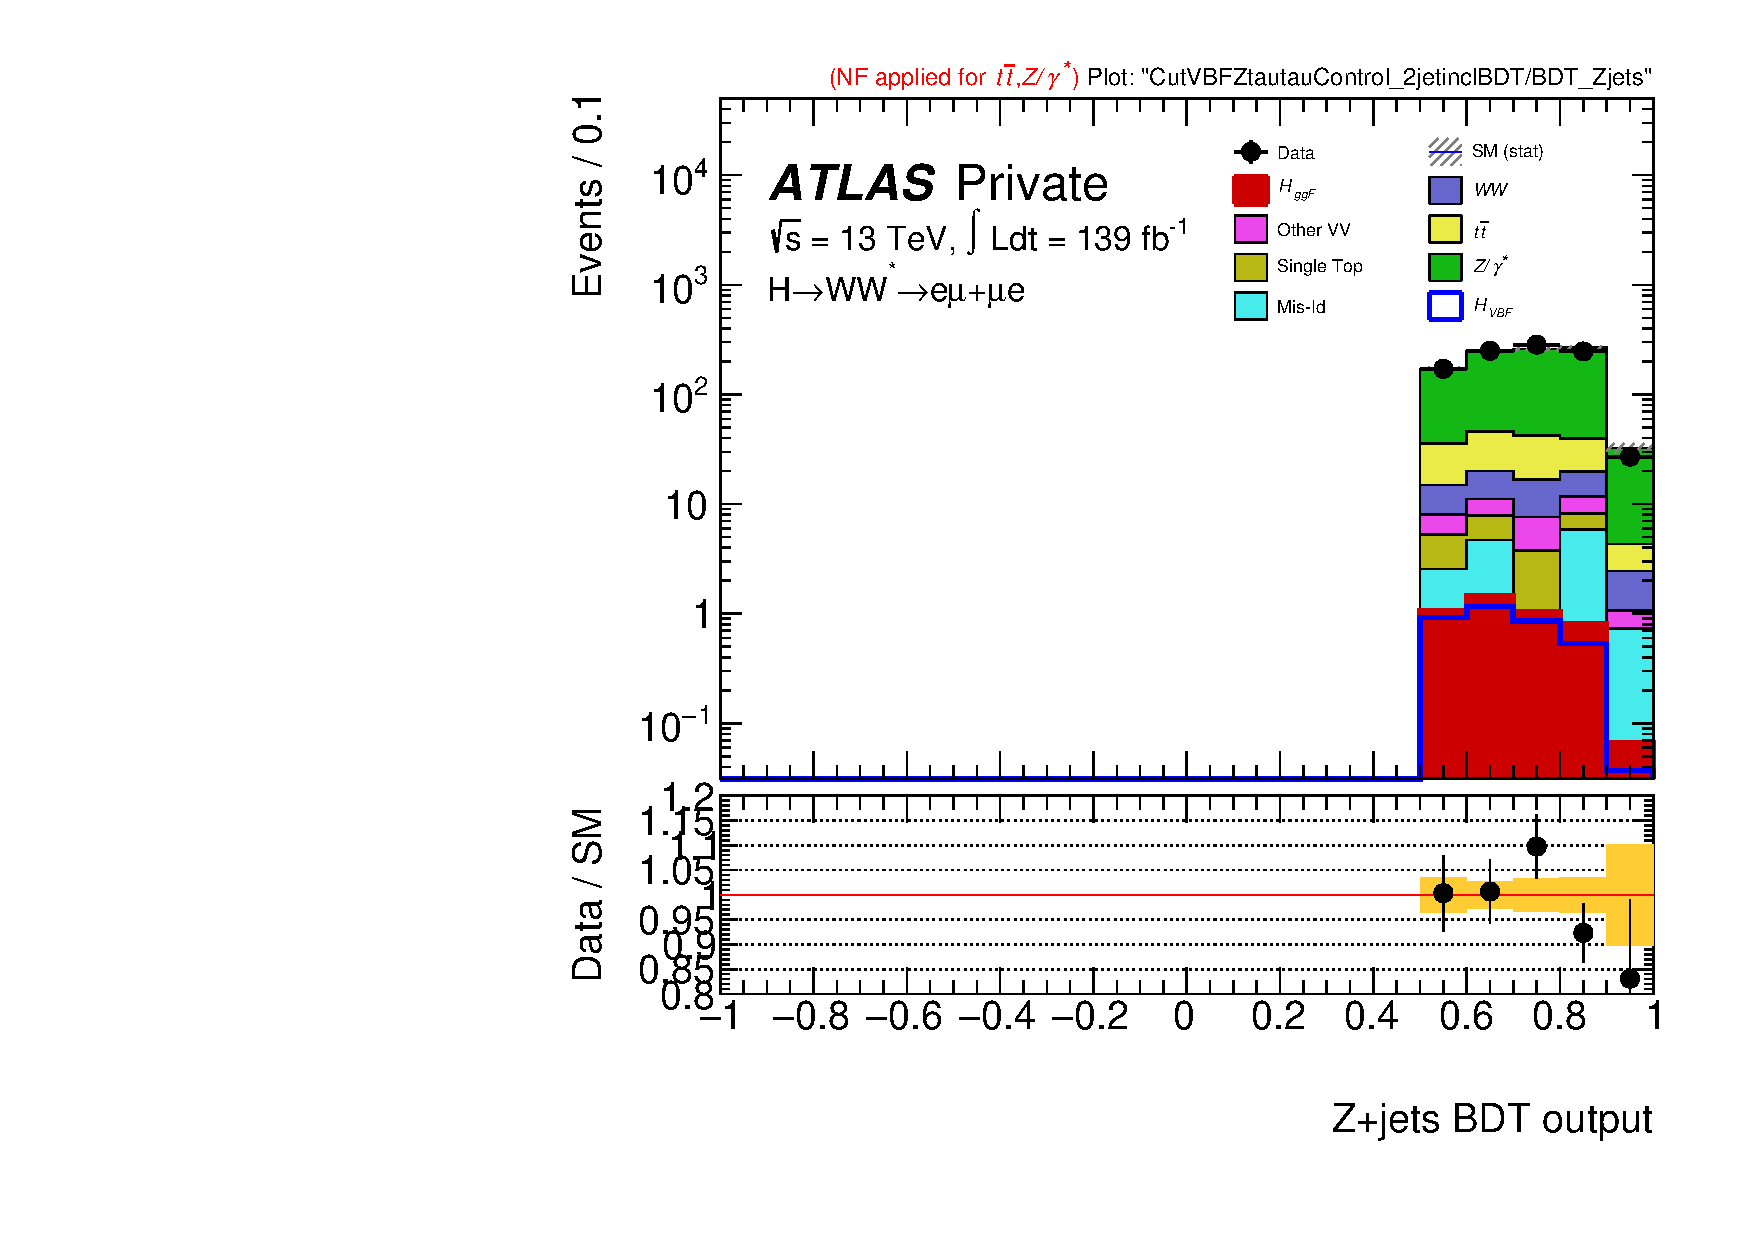
\includegraphics[width=.6\linewidth]{Pictures/run2-emme-CutVBFZtautauControl_2jetinclBDT-BDT_Zjets-log.pdf}
%\caption{Full weighted samples of all signal and background plotted over BDT output distributions in $Z+$jets control region after cut on $Z+$jets BDT}
%\label{fig:ZjetsBDTCR}
%\end{figure}


